\chapter{Dataset Construction}
As opposed to datasets that are widely used in Machine Learning classes at university, in the professional world those are much less frequently available and need to be built on the spot for specific tasks. The major challenge of this project was the data collection part. We needed to determine what was available, what we should use, how to collect it, aggregate it and represent it. 

This protocol was the result of an iterative process of interviews with different stakeholders. Often we had to avoid a given source because initial analysis revealed that the data wasn't usable. The lack of strong documentation of the content of databases certainly made this process longer than expected.

In this chapter we will discuss first how we managed to identify failing \acrshort{cpe}s, we will give an overview of the different measurements that we used to characterise a given \acrshort{cpe}'s health. We will then look at the representation of such measurements to encompass both the notion of time but also to get rid of unwanted idiosyncrasies in the data. We will follow on presenting choices that were made to restrict the dataset and avoid particular cases that lied outside of the scope. Finally, will be presented the strategy that was derived in order to automatise data collection in the most resilient and efficient way.

\section{Identifying Un-heatlhy \acrshort{cpe}}
\subsection{Understanding \acrshort{via}}
Before we get started, it would be useful to define the different keywords that are proper to the way \acrshort{via} stores data. 

When a customer requires technical support, the employee will use \acrshort{via} to service the customer's problems. This software will perform some live measurements to help the employee in the support process. The database is filled by the software but based on the interaction with the agent. 

Whenever a customer calls, a \textbf{session} is started. Each session is composed of multiple \textbf{events} that are launched while the agent interacts with the customer. During a session the agent may start multiple flows. A \textbf{flow} corresponds to the process that the agent follows to diagnose and solve a particular problem that the customer is experiencing. Because he might not know at first which flow is the most appropriate, he will most often start many flows and try to find out which one solves the problem. During a flow execution, the software will emit \textbf{milestones} in order to keep track of the execution of the flow, one for each event. 

Also a \textbf{case} will be created for one or more sessions\footnote{This seems, according to the reporting team, to be a Data Quality issue as first it was intended to be a one to one relationship. But in our scenario we only care to have a unique case for a given session to get the details.} in order to log in an interaction between the customer and the service center. It will give us information regarding the customer details (e.g. the account number that will allow us to recover the Medium Access Control addresses (\acrshort{mac}) of devices that belong to the customer).

\subsection{Protocol to Flag Failing \acrshort{mac}s}
\subsubsection{Labeling Sessions With a Problem}
Our initial goal was to be able to label the problem that is being solved in a given session. Milestones are human readable description of the specific steps of a particular flow, therefore they would be a perfect way for us to attribute a string to a given problem. The challenge was the many events and therefore milestones that are emitted during a particular flow. But also, the many flows that can coexist in a session as explained earlier.

We started by focusing the research on full flows: these are flows that have been completed successfully and yielded the end of the call. In order to detect such flows, we used two flags that are present for each milestone : \texttt{CNT\_INTERACT\_SENT} and \texttt{CNT\_CASE\_SENT}. Whenever one of these two flags (found in table \texttt{SCO.REP\_VIA\_MILESTONE\_V}) is positive then it means that we have found a milestone in a flow that finished the interaction between the agent and the customer. With such strategy we could flag "full" flows.

Then we needed a strategy to choose which milestone to use inside a full flow. This was decided arbitrarily and thanks to the advice of the reporting team. The very first milestone of a full flow would be general enough to give us a problem label. As events inside a session are sequential (not depending on what flow emitted them), we had to look for the minimum event number that had the same flow identifier as the flow determined as "full" in the session. 

\subsubsection{Linking Sessions to Devices}
Another challenge was that we do not store anywhere what is the \acrshort{cpe} that is experiencing problems in the case of the identified sessions. Moreover, it can happen that the customer has multiple \acrshort{cpe}s at home (e.g. one of the boxes commercialised by UPC had trouble to cover a full apartment with Wi-Fi and therefore the company started offering a two-room solution with two Internet-capable devices). 

Because we couldn't find any way to link a particular device to a session we decided to flag all the \acrshort{mac}s of a customer as failing whenever we found a session concerning this particular user. In order to determine what user corresponds to each session we had to join tables \texttt{SCO.REP\_VIA\_CASE\_V} and \texttt{SCO.REP\_VIA\_SESSION\_V} based on \texttt{ID} and \texttt{JOURNAL\_ID} respectively. 

Finally, another problem arose: \acrshort{cpe}s do not necessarily have only one \acrshort{mac}, this is due to the fact that they may use multiple connection interfaces to provide different services (e.g. the Horizon Box provides phone, digital TV and Internet using the network). A first attempt was made to use what is called \textbf{the management \acrshort{mac}} which should be the one that is used in \acrshort{saa} to identify polled \acrshort{cpe}. It yielded poor results (almost no match between management \acrshort{mac}s and those in \acrshort{saa}). Therefore we used another table that was being developed \texttt{DM\_TOPO\_CH.ETL\_STG\_NW\_TOPO\_NODES}. It aims at providing topology information of the network and surprisingly the \acrshort{mac}s extracted from this table yielded much more matches with \acrshort{saa}. The only filtering we had to perform was to focus on nodes with \texttt{topo\_node\_type\_id = 55} as it references \acrshort{cpe} nodes. 

\subsubsection{Ensuring the Exactitude of Our Labeling}
Once we had all these \acrshort{mac}s labeled with a particular problem, we were made aware that a specific session even though it contained a full flow may not have solved the problem of the customer (to be opposed to what is called a \acrfull{ftr}). In order to increase our confidence that the label we gave to the problem  was correct, we had to use yet a different data source \texttt{SCO.REP\_CLY\_INTERACTION\_V}. This table constructed for reporting purposes has a flag called \texttt{FLG\_FTR\_7D\_FLG}. It attempts to check whether the customer called \acrshort{thd} in the following 7 days for the same kind of problem\footnote{The exact logic behind the flag was not available to us but the Business Intelligence team testified that we could trust it as they had already used it in some analysis which offered good results.}. 

This reporting table is built on top of \acrfull{cly}, a service which deals with a more general type of interaction. The challenge was that there is no one-to-one mapping between \acrshort{cly} interactions and \acrshort{via} interactions. We decided that given that the \acrshort{ftr} flag was anyway an estimate we could perform a fuzzy matching between the two. This would still allow us to increase our confidence in the labeling. The assumptions that were formulated were:
\begin{itemize}[topsep=0pt,noitemsep]
	\item The \acrshort{via} case and \acrshort{cly} interaction started on the same day
	\item As \acrshort{via} logs a \acrshort{cly} interaction the timestamp of \acrshort{via} should not be prior to \acrshort{cly} one
	\item Account numbers (the customer) of both match
	\item Employee IDs match as well
\end{itemize}
It happened that this would yield multiple matches and we decided to always take the match from clarify which creation timestamp is the closest to the one in \acrshort{via} as this was the only strategy that we could follow (even checking by hand we couldn't determine the correct match as we had already used all fields that are common between the two sources). 

\subsubsection{Focusing on Certain Problems}
In accordance with the \acrshort{hfc} support expert, we decided to limit our analysis to Internet Problems (which we could do by focusing on Internet Flows in \acrshort{via}) as those would probably be the one to be the most easily identifiable from the \acrshort{saa} data. But also because it would allow us to restrict the analysis to particular \acrshort{cpe}s that have Internet capabilities. 

We realise that this is an arbitrary choice and will discuss later that we may be discarding a lot of detectable problems in the analysis. Nevertheless it also allowed us to focus the research on particular use cases and was validated both with the thesis supervisor (from whom the idea came from originally) and Felix Reisen. 

\section{Characterising \acrshort{cpe}s}
\subsection{Measurement Choices}
\label{subsec:mes_choices}
Choosing the correct measurements to monitor the health of \acrshort{cpe}s required the help of Jonas Staempfli as he had the knowledge regarding how such measurements evolve over time, what normal and abnormal values are, what the time granularity that should be considered to detect problems is and many other tasks specific information. 

As stated earlier, we have at our disposal two types of active nodes in the network that are polled: \acrshort{cpe} and \acrshort{cmts} interface. 

\subsubsection{Available Values}
We started by presenting to the expert all the measurements that we had at hand and asked him to help us choose those that would be the most promising for our prediction task. We have first discussed the measurements available at the \acrshort{cpe} level that were found in \texttt{SAA.CM\_HOUR\_HEALTH}, and we describe in Table~\ref{CPEMes} the features that we decided to keep.

\begin{table}[h]
\begin{center}
\begin{tabular}{c l}
\hline
\textbf{Feature} & \textbf{Description}\\ 
\hline\hline
\texttt{TXPOWER\_UP} & The average upstream transmitting power.\\
\hline
\texttt{RXPOWER\_UP} & The average upstream receiving power.\\
\hline
\texttt{RXPOWER\_DN} & The average downstream receiving power.\\
\hline
\texttt{CER\_DN} & Maximum codeword errors downstream.\\
\hline
\texttt{CER\_UP} & Maximum codeword errors upstream.\\
\hline
\texttt{SNR\_DN} & Sound to noise ratio downstream.\\
\hline
\texttt{PCT\_TRAFFIC\_DMH\_UP} & Percentage of upstream traffic computed as degraded modem hours.\\
\hline
\texttt{PCT\_TRAFFIC\_SDMH\_UP} & Percentage of upstream traffic computed as severally degraded modem hours.
\end{tabular}
\end{center}
\caption{\label{CPEMes}Features at the \acrshort{cpe} level}
\end{table}

Regarding \acrshort{cmts} interfaces we decided to monitor certain measurements because they could give us indications about the group of \acrshort{cpe}s we are looking at. A previous project called Common Path Distortion showed that frequently when a particular node is experiencing problems in a group of nodes then it may affect the whole group. Therefore we repeated the analysis with Jonas regarding which measurements extracted from \texttt{SAA.CMTS\_HOURS\_UPSTREAM\_STATS} (for the upstream channel) and \texttt{SAA.CMTS\_HOURS\_DNSTREAM\_STATS} (respectively for downstream) would serve our purpose. Features that we retained are grouped in Table~\ref{CMTSMes}.

\begin{table}[h]
\begin{center}
\begin{tabular}{c l}
\hline
\textbf{Feature} & \textbf{Description}\\ 
\hline\hline
\texttt{UTILIZATION\_UP} & Maximum percent utilization of upstream.\\
\hline
\texttt{RXPOWER\_UP} & Average power being received by \acrshort{cmts} on interface (upstream).\\
\hline
\texttt{TXPOWER\_UP} & Average power transmitted from CMs on interface (upstream).\\
\hline
\texttt{CER\_UP} & Maximum Codeword Error Ratio for interface (upstream).\\
\hline
\texttt{MS\_UTILIZATION\_UP} & Percent minislot utilization of upstream (upstream).\\
\hline
\hline
\texttt{UTILIZATION\_DN} & Maximum percent utilisation of downstream.\\
\hline
\texttt{RXPOWER\_DN} & Average power being sent by \acrshort{cmts} on interface (downstream).\\
\hline
\texttt{CCER\_DN} & Maximum Corrected Codeword Error Ratio for interface (downstream).\\
\hline
\texttt{CER\_DN} & Maximum Codeword Error Ratio for interface (downstream).\\
\hline
\texttt{AVG\_SNR\_DN} & Average carrier to noise ratio for interface (downstream).\\
\end{tabular}
\end{center}
\caption{\label{CMTSMes}Features at the \acrshort{cmts} interface level}
\end{table}

For each active node all of these measurements are available at a one-hour granularity for 10 full days and we shall discuss in Section~\ref{subsubsec:time_representation} how we used such measurements.

Also we have decided to add, what we referred to as, \textbf{static information}, because they are not time dependent (or at a much greater time granularity with e.g. \texttt{N\_CPE\_BUILDING} presented in Section~\ref{subsubsec:constructed_features}. It will not drastically change over periods that are less than a week except in very particular cases that we considered as minor). These pieces of information are used to either identify the \acrshort{cpe} or track some relevant metrics and are explained in Table~\ref{StaticInfos}.

\begin{table}[h]
\begin{center}
\begin{tabular}{c p{100mm}}
\hline
\textbf{Feature} & \textbf{Description}\\ 
\hline\hline
\texttt{DAY\_0} & As we will explain in Section~\ref{subsubsec:time_representation}, we will aggregate the data at different periods. Therefore each measurements' vector will be relative to a given Day\textsubscript{0}.\\
\hline
\texttt{\acrshort{mac}} & Unique identifier of the \acrshort{cpe}.\\
\hline
\texttt{CLY\_ACCOUNT\_NUMBER} & Unique identifier of the customer in \acrlong{cly}.\\
\hline
\texttt{SAA\_ACCOUNT\_NUMBER} & Unique identifier of the customer in \acrlong{saa} (under Pratheep's advice we decided to keep both account numbers as they could sometimes differ. So far we have yet to find such a case, but it would help us make sure we know how to link the failing \acrshort{cpe} back to a customer).\\
\hline
\texttt{HARDWARE\_MODEL} & Either to facilitate later analysis of the distribution of problems among \acrshort{cpe}s  or to be able to take into consideration what type of hardware we are diagnosing during classification (we suppose that this could influence the values of different features).\\
\end{tabular}
\end{center}
\caption{\label{StaticInfos}Static information collected for each \acrshort{cpe}}
\end{table}

\subsubsection{Constructed Features}
\label{subsubsec:constructed_features}
Aside from these measurements that we arbitrarily selected with the help of the expert, we decided to explore what other measurements could be added in order to characterise as well as possible \acrshort{cpe}s' health. The measurements that we have derived can be found in Table~\ref{CreatedMes}.

\begin{table}[h]
\begin{center}
\begin{tabular}{c p{100mm}}
\hline
\textbf{Feature} & \textbf{Description}\\ 
\hline\hline
\texttt{OFFLINE} & A good indicator of a \acrshort{cpe} experiencing problem could be its status on the network (being online or offline). This information could be derived from \texttt{SAA.CM\_HOUR\_HEALTH} where a \texttt{CM\_STATUS != 8} indicated an offline \acrshort{cpe}.\\
\hline
\texttt{MISS\_*} & Missing values are usually hidden when doing machine learning using imputation, that is we will replace them using some arbitrary values (e.g. mean of the feature, 0, ...). In our case these missing values are missing not at random (MNAR \cite{wiki:mnar}). Later we aggregate these values at the database level and might lose the information about what was missing. So we added \texttt{MISS\_*} that will give for each aggregate (c.f. Section \ref{subsubsec:time_representation}) the percentage of aggregated values that were missing.\\
\hline
\texttt{N\_CPE\_BUILDING} & A given building will have the same signal carrier for all \acrshort{cpe}s. According to the \acrshort{hfc} expert, it could make sense to look at the number of \acrshort{cpe}s that are inside the same building in order to take it into consideration when classifying. Again this information was found in the \texttt{M\_TOPO\_CH.ETL\_STG\_NW\_TOPO\_NODES} table (\textit{Note that this feature is also static}).\\
\end{tabular}
\end{center}
\caption{\label{CreatedMes}Features constructed to enrich existing measurements}
\end{table}


\subsection{Representation Choices}
Now that we have discussed what features could be used for our prediction task, we would like to present the different choices that have been made to properly represent the data. We had to derive different strategies. 

\subsubsection{Linking \acrshort{cmts} Interfaces to \acrshort{cpe}}
We explained in Section~\ref{sec:HFC_archi} that it is somehow challenging to link a \acrshort{cmts} interface to a \acrshort{cpe} as it can change dynamically and very frequently. Therefore we had to design with Jonas Staempfli a workaround to be able to link the \acrshort{cmts} interface measurements presented in Table~\ref{CMTSMes} with \acrshort{cpe} measurements presented in table~\ref{CPEMes}. The most coherent grouping we found was to use the service group as a logical grouping of \acrshort{cpe}s. 

Therefore the \acrshort{cmts} interfaces measurement were averaged over all the interfaces of a given service group and presented as the measurements at the service group level. We found the mapping between interfaces in table \texttt{DM\_DIM.ETL\_STG\_TOPO\_CMTS2NODE}.

\subsubsection{Decreasing Group Specificities}
Then we wanted to make sure that we could work with relative data. While discussing with different stakeholders at UPC, we discovered that it was very common to have a group of \acrshort{cpe}s with abnormally high values for certain measurements even though they were not experiencing any issues.

This drove us to scale the \acrshort{cpe} features in each logical group (the Service Group) in order to get rid of these specificities and hopefully obtain relative values that would be comparable between \acrshort{cpe}s in different locations of the network tree. 

\subsubsection{Including the Time Dimension of Failures}
\label{subsubsec:time_representation}
We cannot detect failure at the exact time they happen. This is why we need to collect data over an extended period of time for each \acrshort{cpe} failure such that we give our classifier the history of the \acrshort{cpe}s' behavior to let it flag the outlying values. 

Discussing with the \acrshort{hfc} support expert, he first advised us not to consider a time granularity that would be too fine. Indeed health measurements of \acrshort{cpe}s can 'flap' without any real connection to a potential problem (e.g. due to electromagnetic fields or change in temperatures). 

Also as we already have a large number of values it would make sense not to keep all time measurements but rather to aggregate these measurements over different time granularities:
\begin{itemize}
	\item Last 24 hours: this was what we estimated as the most probable time when failure happened (usually customers would not wait that long in case of service degradations before reaching out). Over the last 24 hours we considered 6 hour windows on which we averaged all measurements.
	\item Last 6 days: this was considered as the maximum amount of time a customer could wait before calling \acrshort{thd}. For this period we took a longer averaging window of 1 day to limit the resulting number of features (this is a tradeoff that will be discussed in final parts).
\end{itemize}

Then we also found out that what we are really interested in isn't the absolute value of a measurement but rather its evolution over time. Therefore we decided to present a given time aggregate as a difference between the current aggregate and the previous one in order to only display the evolution of these aggregates over time. 

Therefore if we consider a measurement $x$ and denote by $x^d_i$ for $i \in \{0,..23\}$ and $d \in \{0,...,-5\}$  the polled version of x at the $i^\text{th}$ hour of day $d$ (where d is relative to Day\textsubscript{0}). We will construct : 

\begin{equation}
\begin{cases}
	\hat{x}_{6h} &= (x^0_{23}+...+x^0_{18})/6 - (x^0_{17}+...+x^0_{12})/6\\
	\hat{x}_{12h} &= (x^0_{17}+...+x^0_{12})/6 - (x^0_{11}+...+x^0_{6})/6\\
	\hat{x}_{18h} &= (x^0_{11}+...+x^0_{6})/6 - (x^0_{5}+...+x^0_{0})/6\\
\end{cases}
\end{equation}

This means for example that $\hat{x}_{18h}$ is the average of the 6 hour window that started 18h before midnight on Day\textsubscript{0} represented as the difference with respect to the previous window. To ease up comprehension, we present the operation on Figure~\ref{6h_agg}.

\begin{figure}[ht]
    \begin{center}
    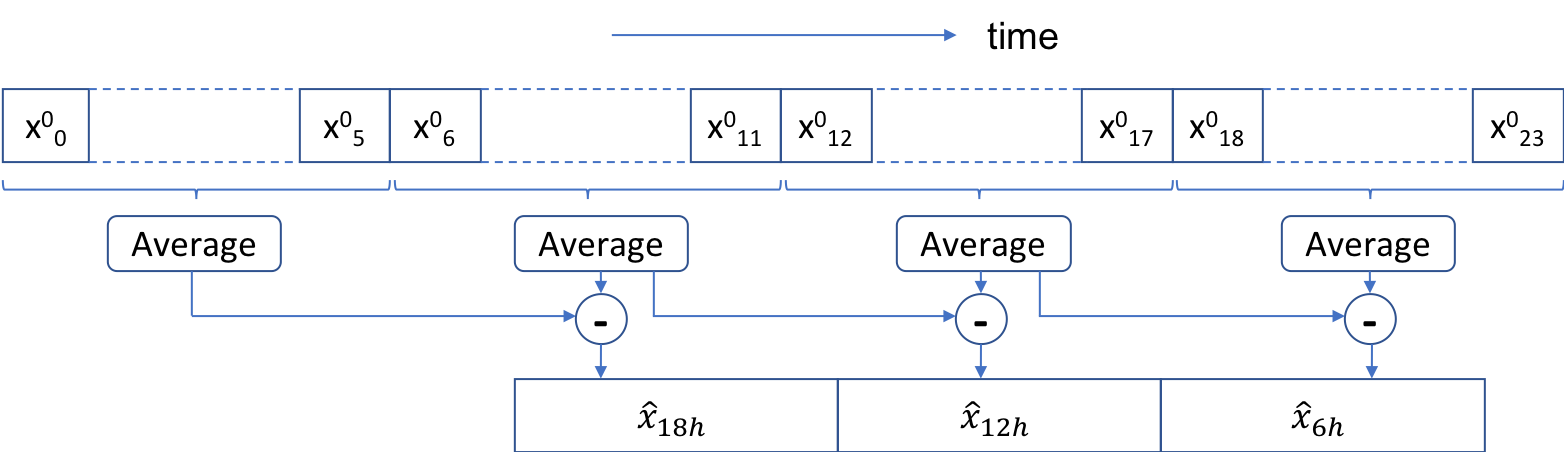
\includegraphics[width=1\linewidth]{6h_aggregation}
    \end{center}
    \caption{The aggregation over the last 24 hours with 6 hour window averaging and relativisation of averages with respect to the past aggregate}
    \label{6h_agg}
\end{figure}


And then we construct:

\begin{equation}
\begin{cases}
	\hat{x} &= (x^0_{23}+...+x^0_{0})/24\\
	\hat{x}_{1d} &= (x^0_{23}+...+x^0_{0})/24 - (x^1_{23}+...+x^1_{0})/24\\
	...\\
	\hat{x}_{5d} &= (x^4_{23}+...+x^4_{0})/24 - (x^5_{23}+...+x^5_{0})/24\\
\end{cases}
\end{equation}

The principle is identical to what we do with 6 hour averages.

By allowing these two granularities we have constructed a vector that gives us the history of values over multiple days and hours. It is important to note that not all measurements were represented as relative differences w.r.t. their previous average. Regarding \texttt{OFFLINE} and \texttt{MISS\_*} it would not make sense to make such relative\footnote{Because their magnitude actually matter more than their evolution on the long run.}, so we simply represented them as their averages (therefore for the last 24 hours they are represented as 4 values e.g. \texttt{OFFLINE\_PCT\_6H}, \texttt{OFFLINE\_PCT\_12H}, \texttt{OFFLINE\_PCT\_18H}, \texttt{OFFLINE\_PCT\_24H} which are simply the averages from the first up to the 4th furthest 6h window).

\section{Restricting the Dataset: Offline \acrshort{cpe}s}
\subsubsection{Outliers Detection}
During our initial analysis we realised that offline \acrshort{cpe}s wouldn't have any polled values and that would be a problem. With rising ecological concerns and energetic awareness, it seems like many people turn off their electronic at night. We didn't have any simple way to verify this gut feeling so we decided to prevent it by filtering our dataset. Nevertheless we couldn't take out all offline \acrshort{cpe}s as this could be already eliminating outliers that are indeed failing \acrshort{cpe}s. 

We had 10 days of data in \acrshort{saa} that we could use in order to detect these outliers. Using the \texttt{OFFLINE} feature that we constructed for each measurement, we could compute for each \texttt{HARDWARE\_MODEL} what would be standard offline times. In order to find such standard offline time we looked at the 99\textsuperscript{th} percentile (the value that will separate the population into a 99\% that we keep and 1\% we discard) of the offline frequency at a given hour of the day computed over all the days of history. To put things simply with 10 days of data, we look at the measurements made at 3am. Our assumption is that if someone turns off their \acrshort{cpe} during the night then he will have a frequency of being offline at 3am of $100\%$ which will be detected with respect to a \acrshort{cpe} that has an issue once in a while at 3am causing it to be offline. We took out any \acrshort{cpe} that was an outlier for any given hour. 

We made it relative to a particular model as some models may be more prone to errors causing them to be more offline than others, the underlying desire was to compare only pieces of hardware that are comparable. 

\subsubsection{Accidental Discovery: Automatic Deep Sleep Mode}
While performing this analysis we observed surprising results. We plotted for each type of hardware model the cutoff values that were obtained. Because the 99\textsuperscript{th} percentile was a bit too discriminative to see much, we looked at the 80\textsuperscript{th}. As it can be observed on Figure~\ref{offline}, the cutoff values for Media Box and Horizon Box are alarmingly high. It means that for such devices most of the population is offline during most of the day. 

\begin{figure}[ht]
    \begin{center}
    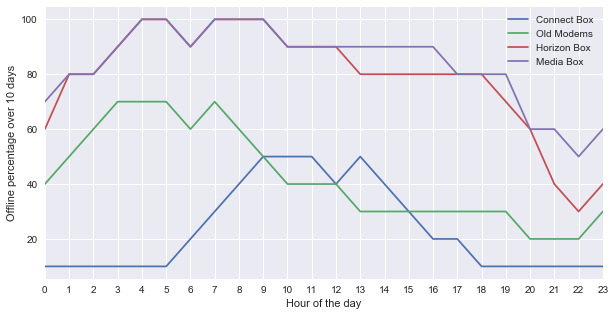
\includegraphics[width=1\linewidth]{offline}
    \end{center}
    \caption{80\textsuperscript{th} centile per hour of the day by Hardware type in terms of offline percentage computed over 10 days of history}
    \label{offline}
\end{figure}

By presenting these results to different stakeholders and mostly the \acrshort{hfc} support team we discovered that we had forgotten about a particular feature of most recent \acrshort{cpe}s: automatic deep sleep mode. UPC is obligated by law on all new models to automatically turn off the \acrshort{cpe} if it hasn't been used for a given period of time. Also this feature is enabled by default and hence will affect most of the models that have it built in. These models had to be taken out of our analysis as they would present a lot of missing measurements and possibly give false training patterns to our model.

\begin{table}[h]
\begin{center}
\begin{tabular}{c l r r}
\hline
\textbf{Type} & \textbf{\texttt{Hardware Model}} & \textbf{Offline \%} & \textbf{\acrshort{saa} \%}\\ 
\hline\hline
\multirow{3}{*}{Horizon Box} 		& \textbf{HORIZON HD RECORDER}					& $27.23\%$ 			& $\mathbf{18.80\%}$\\
									& \textbf{HORIZON HD RECORDER (G7401)} 			& $20.95\%$ 			& $\mathbf{15.07\%}$\\
									& HORIZON VSC									& $0\%$ 				& $0\%$\\
\hline						
Connect Box							& \textbf{CONNECT BOX CH7465LG COMPAL}			& $23.42\%$ 			& $\mathbf{41.16\%}$\\
\hline
\multirow{6}{*}{Mediabox} 			& MEDIABOX RECEIVER THOMSON DC152UPC 			& $0.04\%$ 				& $0.02\%$\\
									& MEDIABOX HD PHILIPS DCR8111/03 				& $0.01\%$ 				& $0\%$\\
									& MEDIABOX RECORDER HD CISCO						& $1.43\%$ 				& $0.74\%$\\
									& MEDIABOX RECORDER HD CISCO 8685				& $4.70\%$ 				& $3.05\%$\\
									& \textbf{MEDIABOX HD PACE DCR7111}				& $12.83\%$ 			& $\mathbf{7.02\%}$\\
									& MEDIABOX HD PHILIPS DCR7101/03					& $0.04\%$ 				& $0.02\%$\\
\hline
\multirow{6}{*}{Old Modems} 			& UBEE EVM3236 (ED 3.0) - CPE 					& $2.13\%$ 				& $2.94\%$\\
									& UBEE EVM3206 (ED 3.0) - CPE 					& $1.46\%$ 				& $1.72\%$\\
									& WLAN MODEM TC7200 - CPE						& $2.79\%$ 				& $4.62\%$\\
									& WLAN MODEM EVW3226 - CPE						& $0.56\%$ 				& $0.86\%$\\
									& WLAN MODEM TC7200 V2 - CPE						& $1.05\%$ 				& $1.89\%$\\
									& WLAN MODEM TWG870 - CPE						& $1.23\%$ 				& $1.92\%$\\
\hline 
\multirow{13}{*}{FTTH (Left out)} 	& FTTH\_CPE\_UBEE EVM3206 (ED 3.0) - CPE 		& $0\%$ 				& $0\%$\\
									& FTTH\_CPE\_UBEE EVM3236 (ED 3.0) - CPE 		& $0\%$ 				& $0\%$\\
									& FTTH\_CPE\_CONNECT BOX CH7465LG COMPAL			& $0.04\%$ 				& $0.08\%$\\
									& FTTH\_CPE\_HORIZON HD RECORDER					& $0.03\%$ 				& $0.02\%$\\
									& FTTH\_CPE\_HORIZON HD RECORDER (G7401)			& $0.04\%$ 				& $0.03\%$\\
									& FTTH\_CPE\_MEDIABOX HD PACE DCR7111			& $0.01\%$ 				& $0.01\%$\\
									& FTTH\_CPE\_MEDIABOX RECORDER HD CISCO 8685	& $0.01\%$ 				& $0\%$\\
									& FTTH\_CPE\_WLAN MODEM TC7200 V2 - CPE			& $0\%$ 				& $0\%$\\
									& FTTH\_CPE\_WLAN MODEM TC7200 - CPE				& $0\%$ 				& $0\%$\\
									& FTTH\_CPE\_WLAN MODEM TWG870 - CPE				& $0\%$ 				& $0\%$\\
									& FTTH\_CPE\_MEDIABOX HD PHILIPS DCR7101/03		& $0\%$ 				& $0\%$\\
									& FTTH\_CPE\_WLAN MODEM EVW3226 - CPE			& $0\%$ 				& $0\%$\\
									& FTTH\_CPE\_MEDIABOX RECORDER HD CISCO			& $0\%$ 				& $0\%$\\

\end{tabular}
\end{center}
\caption{\label{CPEProportions}Internet Capable \acrshort{cpe}s, their proportion among \acrshort{saa} measurements, and the proportion among all measurements from such \acrshort{cpe}s marking the \acrshort{cpe} as offline. (Note that percentages have been rounded.)}
\end{table}

In the table~\ref{CPEProportions}, we have described all Internet-capable \acrshort{cpe}s and highlighted those that have the highest frequency in the dataset. According to Business Intelligence, the FTTH \acrshort{cpe} can be left out of the analysis as they do not correspond to hardware used by customers. Horizon Box and Media Box must be left out of the analysis as stated above due to their deep sleep mode. Therefore the only \acrshort{cpe}s that we considered in the analysis were the Connect Box and Old modems.

\section{Collecting the Data}
The restrictions on the type of \acrshort{cpe} analysed combined with the way we identify failing \acrshort{cpe}s yielded approximately $500,000$ \acrshort{mac}s considered every day and an average of $112$ daily failing \acrshort{cpe}s (representing $0.224\%$ of this analysed population).

So far we discussed the construction of vectors composed of five days of history. We will see in the following section that practically this construction was implemented in a different way for optimisation reasons. We shall also discuss the different techniques that have been used to make this data collection reproducible and automatised. 

\subsection{Collecting Over Multiple Days}
\label{subsec:collecting}
As stated earlier, \acrshort{saa} only keeps 10 days of history. Therefore we could not build a representative dataset from these 10 days of history (one of our concerns being that we would like to balance the dataset to improve training). Therefore we had to collect over multiple days to iteratively increase the dataset. That required some engineering in the way we collect data.

\subsubsection{Collection Timeline}

\begin{figure}[ht]
    \begin{center}
    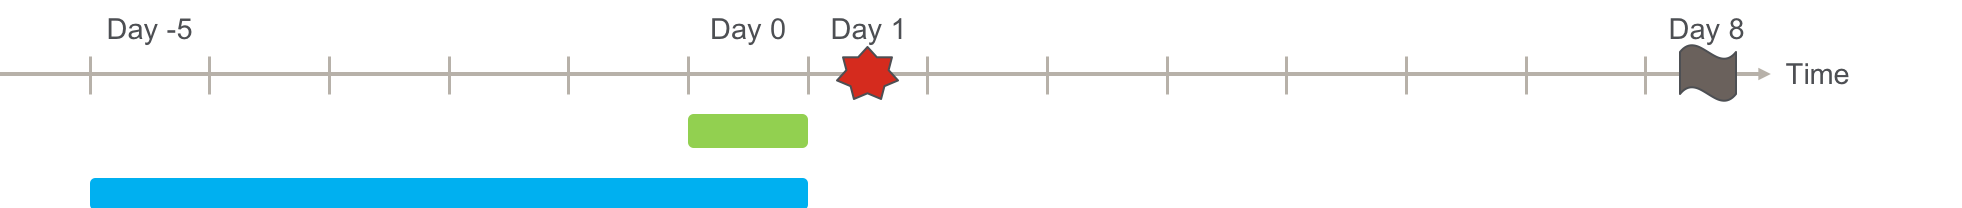
\includegraphics[width=1\linewidth]{timeline}
    \end{center}
    \caption{Graphical representation of the timeline of how the vectors are constructed}
    \label{timeline}
\end{figure}

Figure~\ref{timeline} illustrates how health measurements are collected. On Day\textsubscript{0} as represented by the green Label we collect the data with our 6-hour window averages while from Day\textsubscript{-5} to Day\textsubscript{0} we also aggregate with 1 day windows. On Day\textsubscript{1} we monitor \acrshort{via} calls for potential failure (so that we can, using health measurements collected on Day\textsubscript{0}, predict whether the \acrshort{cpe} will fail the following day). In order to validate our labeling of the problem happening on Day\textsubscript{1} we need to wait Day\textsubscript{9} to make sure that the \acrshort{ftr} flag has been set as we have explained it previously. 

Therefore when collecting the data on a given day $d$, we can collect vectors that have a $\text{Day\textsubscript{0}} = d-1$ (as represented in our \acrfull{plsql} packages by the variable \texttt{var\_day\_0}). We do not flag vectors to determine whether they are failing or not at collection time. Indeed we have only a short history available to construct these vectors. But also we need to wait the \acrshort{ftr} flag to be set before we can label them. Therefore on day $d$, we collect pieces of information that we extract from \acrshort{via} such that for such vectors $\text{Day\textsubscript{0}} = d-8$ (respectively represented by \texttt{var\_via\_day\_0}). We will discuss at a later stage how we can join these two sources.


\subsubsection{Efficiency}
\paragraph{\acrshort{dmp} and \acrshort{dmt}}
As we started developing the project, we used \acrfull{dmp} as a playground but soon enough we were told that this server was to be used only for production-ready software. Indeed there exist a second server dedicated to testing called \acrfull{dmt}. This server, on the other hand, provides much less computational power but also allows us to store any amount of data that we may need to store for the sake of this project. Hence to leverage the power of \acrshort{dmp} and the storage capabilities of \acrshort{dmt} we had to develop a strategy: doing aggregations on the production data mart and storing the results on the test environment.


\paragraph{Rolling Window Mechanism - \acrshort{dmp}}
Our aim was to avoid as much as possible duplicated computation and to efficiently use the resources that are available for the \acrshort{poc}'s development. That's where we derived a rolling window mechanism to iteratively construct the vectors. Put simply, every day we compute the aggregates and wait until we have enough aggregates to build a full vector (which involves computing the differences between aggregate as stated in Section~\ref{subsubsec:time_representation}). 

We have created, on \acrshort{dmp}, four \textbf{buffer tables}. These will temporarily hold data in order to be later assembled into five days vectors:
\begin{itemize}
	\item \texttt{VECTOR}\footnote{We won't state the schema into which we are but for the duration of the \acrshort{poc} all work resided in \texttt{HUMOREAU}.}: holds what we have defined as static information as well as the 6h window averages for the past 24 hours for Day\textsubscript{0} $= \texttt{var\_day\_0}$.
	\item \texttt{DAILY\_AVG\_DAY\_0}: stores the measurements of Day\textsubscript{0} aggregated on a daily basis for all Day\textsubscript{0} $\in \{\text{\texttt{var\_day\_0}}-1,\text{\texttt{var\_day\_0}}\}$
	\item \texttt{DAILY\_AVG\_DIFFS}: stores the daily average differences (except for features that are static, as described in Section \ref{subsec:mes_choices}, that are stored as averages) between Day\textsubscript{0} and Day\textsubscript{-1} for all Day\textsubscript{0} $\in \{\text{\texttt{var\_day\_0}}-4,...,\text{\texttt{var\_day\_0}}\}$
	\item \texttt{VIA\_MACS}: holds the \acrshort{mac}s that have been identified as failing on Day\textsubscript{0}$=\text{\texttt{var\_via\_day\_0}} = \text{\texttt{var\_day\_0}} - 8$. Indeed it holds more details about such \acrshort{mac} that could be useful for future reality checks (\texttt{MAC}, \texttt{DAY\_0}, \texttt{MILESTONE\_NAME}, \texttt{CASE\_ID},\texttt{SESSION\_ID},\texttt{EMP\_ID}, \texttt{CLY\_ACCOUNT\_NUMBER}, \texttt{CASE\_START\_T}, \texttt{PROCESS\_FLOW}, \texttt{FLG\_FTR\_7D\_FLG},\texttt{FLG\_FTR\_0D\_FLG}).
\end{itemize}
Note that each table is uniquely identified by the pair (\texttt{DAY\_0},\texttt{MAC}) which will allow us at a later stage to join these chunks of information. Also note that \texttt{VIA\_MACS} contains information about days that are 8 days earlier than the earliest of the first 3 tables as explained above.

Every day we update the content of these tables in order to always satisfy the four properties we just defined. In order to perform these operations, we have introduced 33 \textbf{intermediary tables} that allow us to temporarily hold computations that are necessary to fill in buffer tables. Their content is purged at the end of each run. Given that the different steps regarding how we fill intermediary tables have been documented and that the general procedure has been explained we didn't judge necessary to explain it in detail here.

To update the content of buffer tables the package will, for Day\textsubscript{0} being the $ \text{\texttt{var\_day\_0}}=\text{current day} - 1$:
\begin{enumerate}
\item Find the static information and compute the 6 hour averages of the chosen measurements over \texttt{var\_day\_0}. Insert them into \texttt{VECTOR}. Delete the entries in \texttt{VECTOR} that correspond to an older day.
\item Aggregate the 6-hour window averages into daily averages. And insert them into \texttt{DAILY\_AVG\_DAY\_0}. It will then also delete the entries in the table that are the eldest (that is entries for which $\text{Day\textsubscript{0}}=\text{\texttt{var\_day\_0}}-2$).
\item Use the daily averages in \texttt{DAILY\_AVG\_DAY\_0} for $\text{Day\textsubscript{0}}=\text{\texttt{var\_day\_0}}$ and $\text{Day\textsubscript{0}}=\text{\texttt{var\_day\_0}}-1$ in order to construct the differences between Day\textsubscript{0} and Day\textsubscript{-1}. It will then insert them into \texttt{DAILY\_AVG\_DIFFS}. Again it will delete the content of the table that is the eldest, that is entries which $\text{Day\textsubscript{0}}=\text{\texttt{var\_day\_0}}-5$.
\item Finally, it fills in the \acrshort{mac}s that have been identified as failing for $\text{Day\textsubscript{0}}=\text{\texttt{var\_day\_0}}-8$ and will delete the old content of the table that is a day older. 
\end{enumerate}

\paragraph{Rolling Window Mechanism - \acrshort{dmt}}
\acrshort{dmt} will hold the tables that store the unloaded versions of \acrshort{dmp} once the vectors have been materialised:
\begin{itemize}
	\item \texttt{VECTOR\_FIVE\_DAYS\_II}\footnote{the suffix of the table indicates it is the second iteration of such table and we will explain why in Section~\ref{subsec:data_sampling}.}: holds all 5 days vectors with the components and representation that were discussed earlier.
	\item \texttt{VIA\_MACS}: holds all the information that is collected in the homonym table created on \acrshort{dmp} for all Day\textsubscript{0} since we started collecting data.
\end{itemize}

Again each table entry is uniquely identified by the pair (\texttt{DAY\_0},\texttt{MAC}). The update that runs every day will happen after \acrshort{dmp} table content has been successfully completed (we should explain how we synchronise between these two tables in the following paragraph). In order to perform the update, the package will:
\begin{enumerate}
	\item Construct a flat vector with the whole content of \texttt{DAILY\_AVG\_DIFFS}, such that for each (\texttt{DAY\_0},\texttt{MAC}) we have the daily average differences of the 5 previous days in a single vector.
	\item Compute the differences between the 6h window averages in \texttt{VECTOR} as explained in Section~\ref{subsubsec:time_representation}. into one vector for each pair (\texttt{DAY\_0},\texttt{MAC}). Prepend each vector with the static information that can also be found in \texttt{VECTOR}.
	\item Finally, it can join everything we have just constructed into a single vector with the daily average for \texttt{DAY\_0} from \texttt{DAILY\_AVG\_DAY\_0} as we desired and insert them in \texttt{VECTOR\_FIVE\_DAYS\_II}.
	\item The last step is to dump all the content of \acrshort{dmp}'s \texttt{VIA\_MACS} into the homonym table in \acrshort{dmt}.
\end{enumerate}

\paragraph{Automatisation: Checks and Logging}
Because these two packages have to be executed daily (even on non-working days) it would be desirable not to have to launch execution manually every time. 

In order to synchronise the two packages, we had to design a way to log events of each procedure. The main challenge is that whenever a procedure fails to update the state of a database then the whole state of the database is rolled back. Therefore we created a logging table (\texttt{LOG\_TABLE} on each data mart). These are updated using autonomous transactions. It means that the transaction itself has independent commit with respect to the rest of the procedure (allowing us to keep a trace of what happened even when the state is rolled back). The behavior of this log table was implemented in \texttt{CPE\_FAILURE\_ERROR\_LOG}. It will contain:
\begin{itemize}[noitemsep]
	\item Execution times of each part of the package.
	\item Insertion counts into intermediary and buffer tables.
	\item Potential errors that happened during execution (either using custom made error messages for expected errors or using \acrshort{sql} error messages)
	\item Flags allowing to know whether the full procedure was successful. 
\end{itemize}		

But to automatise execution we needed a couple of tricks to ensure correctness of collected data. First, each package before being executed respectively on the production and test environment will perform multiple checks:
 \begin{itemize}
	\item \acrshort{dmp}:  \begin{itemize}[noitemsep,topsep=0pt]
					\item Check the state of the database: the correct dates are in the buffer tables w.r.t the Day\textsubscript{0} that will be computed (because it is a rolling window if the past iteration wasn't successful or didn't happen we cannot compute the current one).
					\item Check that the last run performed without errors (by verifying that the log table is empty as it should be emptied by the \acrshort{dmt} package in case of a successful run).
					\item Make sure that intermediary computations yield non-empty results when they shouldn't (it can happen that some table are empty e.g. \acrshort{via} can yield no identified failing \acrshort{cpe}s which shouldn't raise an error).
				\end{itemize}
	\item \acrshort{dmt}: 	\begin{itemize}[noitemsep,topsep=0pt]
					\item Make sure that \texttt{var\_day\_0} is strictly posterior to what we have already computed.
					\item Ensure that the \acrshort{dmp} procedure has executed correctly (if so it will dump the content of the log table in production into test after having reset it).
					\item Again it will make sure that content is indeed inserted when expected (no empty insertion count)
				\end{itemize}
\end{itemize}	

These tricks allowed us to make the two procedures into a job that could be run automatically using SAP and that would send us an email depending on the success or failure of the job. 

\subsection{Data Sampling}
\label{subsec:data_sampling}

Because we decided to keep collecting data as long as we could in order to build a more comprehensive dataset, the size of the original \texttt{VECTOR\_FIVE\_DAYS} table became quickly concerning. Running queries on such a big table\footnote{When it contained 30 days of data, the table had a size of 210 GB, mostly due to the fact that every day we insert 500'000 entries of 291 columns.} was taking prohibitively too much time. 

It was not an option to import the whole constructed dataset on the data analysis machine (a personal computer), first of all, because of its size but also because any way we were going to subsample the healthy class in order to train our models. Therefore we derived a technique to be able to sample from this table easily at the database level. 

Upon insertion we create a \texttt{SEQ\_ID} that is automatically generated by \acrshort{sql} such that it will be incremented at each insertion (what is called an \texttt{AUTO\_INCREMENT} column). Because of some limitation from Oracle, this \texttt{SEQ\_ID} is ensured to be strictly increasing but not necessarily sequential (though it should be very rare that a gap appears between such IDs). By making \texttt{SEQ\_ID} as a key on the table, we can be sure that obtaining entries with a particular value in such field will be done in an optimised way. This is why the table \texttt{VECTOR\_FIVE\_DAYS} has evolved into \texttt{VECTOR\_FIVE\_DAYS\_II}.

In order to sample from the dataset (as implemented in \texttt{SAMPLE} on the \acrshort{dmt} package):
\begin{enumerate}
	\item We join \texttt{VIA\_MACS} with \texttt{VECTOR\_FIVE\_DAYS\_II} in order to obtain the vectors corresponding to unhealthy \acrshort{mac}S.
	\item Then we randomly sample from \texttt{VECTOR\_FIVE\_DAYS\_II} by using a random series of \texttt{SEQ\_ID} ranging on the full range of those\footnote{To make execution faster we decided to tolerate collisions between the healthy and unhealthy \acrshort{mac}s. That means that when the selected sampling size is $n$ we might end up with slightly less than $n$ entries. Nevertheless given the relative small size of the 'sick' class w.r.t. the 'healthy' one, collisions are sufficiently unlikely to be ignored.}. 
	\item We join the two tables that were obtained from the previous steps and insert the result into \texttt{SAMPLED\_VECTOR} residing in the test environment. 
\end{enumerate}

That technique allowed us to efficiently sample the dataset to fully utilise the 'sick' class and subsample the healthy class to facilitate further analysis.

\subsection{Initialisation}
Finally, in order to allow the project to be restarted at a later time, we decided to provide the necessary packages that would allow automatic initialisation of the state of the tables but also the creation of all the tables that are used by the data collection packages. 

Two distinct versions of the \texttt{CPE\_FAIL\_DETECTION\_POC\_INIT} packages addressing the initialisation of the production and test environment. Both versions have in common that they will first create all the necessary tables (including log tables). These additional packages had to be created as a package will not compile if it references tables that do not exist, hence if the initialisation procedure would be in the same package as the data collecting procedures it would be impossible to initialise tables once they have been dropped.

As we have already explained in great details, \acrshort{dmp} package works iteratively as it needs the state of the buffer tables to be initialised. Therefore, once the \texttt{CPE\_FAIL\_DETECTION\_POC\_INIT.INITIALISE} has been executed we still need to run \texttt{CPE\_FAIL\_DETECTION\_POC.INIT}. Together these procedures will initialise the state of \acrshort{dmp} tables such that a call to \texttt{CPE\_FAIL\_DETECTION\_POC.MAIN\_PROC} (the procedure that collects the data) can be done on the same day. 

Each package has been documented inline in order to explain exact steps that must be followed to allow data collection to be restarted in order to ensure the reproducibility but also to support further development of the project.

\vspace{1 \baselineskip} 
This chapter summarises the most important challenge of this project. Lots of effort has been put in data collection. It required to learn more about the company and fight the obscurity around data sources. This whole process had to be implemented in \acrshort{plsql} which represented yet another overhead but was necessary to comply with UPC's data architecture. Data was chosen and represented based on intuitions and advices from different stakeholders in the company. Finally, the process was automatised to facilitate our work but also to ensure knowledge acquired during this phase would be easily transferable for further development. 